%% LyX 2.0.6 created this file.  For more info, see http://www.lyx.org/.
%% Do not edit unless you really know what you are doing.
\documentclass{article}\usepackage{graphicx, color}
%% maxwidth is the original width if it is less than linewidth
%% otherwise use linewidth (to make sure the graphics do not exceed the margin)
\makeatletter
\def\maxwidth{ %
  \ifdim\Gin@nat@width>\linewidth
    \linewidth
  \else
    \Gin@nat@width
  \fi
}
\makeatother

\IfFileExists{upquote.sty}{\usepackage{upquote}}{}
\definecolor{fgcolor}{rgb}{0.2, 0.2, 0.2}
\newcommand{\hlnumber}[1]{\textcolor[rgb]{0,0,0}{#1}}%
\newcommand{\hlfunctioncall}[1]{\textcolor[rgb]{0.501960784313725,0,0.329411764705882}{\textbf{#1}}}%
\newcommand{\hlstring}[1]{\textcolor[rgb]{0.6,0.6,1}{#1}}%
\newcommand{\hlkeyword}[1]{\textcolor[rgb]{0,0,0}{\textbf{#1}}}%
\newcommand{\hlargument}[1]{\textcolor[rgb]{0.690196078431373,0.250980392156863,0.0196078431372549}{#1}}%
\newcommand{\hlcomment}[1]{\textcolor[rgb]{0.180392156862745,0.6,0.341176470588235}{#1}}%
\newcommand{\hlroxygencomment}[1]{\textcolor[rgb]{0.43921568627451,0.47843137254902,0.701960784313725}{#1}}%
\newcommand{\hlformalargs}[1]{\textcolor[rgb]{0.690196078431373,0.250980392156863,0.0196078431372549}{#1}}%
\newcommand{\hleqformalargs}[1]{\textcolor[rgb]{0.690196078431373,0.250980392156863,0.0196078431372549}{#1}}%
\newcommand{\hlassignement}[1]{\textcolor[rgb]{0,0,0}{\textbf{#1}}}%
\newcommand{\hlpackage}[1]{\textcolor[rgb]{0.588235294117647,0.709803921568627,0.145098039215686}{#1}}%
\newcommand{\hlslot}[1]{\textit{#1}}%
\newcommand{\hlsymbol}[1]{\textcolor[rgb]{0,0,0}{#1}}%
\newcommand{\hlprompt}[1]{\textcolor[rgb]{0.2,0.2,0.2}{#1}}%

\usepackage{framed}
\makeatletter
\newenvironment{kframe}{%
 \def\at@end@of@kframe{}%
 \ifinner\ifhmode%
  \def\at@end@of@kframe{\end{minipage}}%
  \begin{minipage}{\columnwidth}%
 \fi\fi%
 \def\FrameCommand##1{\hskip\@totalleftmargin \hskip-\fboxsep
 \colorbox{shadecolor}{##1}\hskip-\fboxsep
     % There is no \\@totalrightmargin, so:
     \hskip-\linewidth \hskip-\@totalleftmargin \hskip\columnwidth}%
 \MakeFramed {\advance\hsize-\width
   \@totalleftmargin\z@ \linewidth\hsize
   \@setminipage}}%
 {\par\unskip\endMakeFramed%
 \at@end@of@kframe}
\makeatother

\definecolor{shadecolor}{rgb}{.97, .97, .97}
\definecolor{messagecolor}{rgb}{0, 0, 0}
\definecolor{warningcolor}{rgb}{1, 0, 1}
\definecolor{errorcolor}{rgb}{1, 0, 0}
\newenvironment{knitrout}{}{} % an empty environment to be redefined in TeX

\usepackage{alltt}
\usepackage[sc]{mathpazo}
\usepackage[T1]{fontenc}
\usepackage{geometry}
\geometry{verbose,tmargin=2.5cm,bmargin=2.5cm,lmargin=2.5cm,rmargin=2.5cm}
\setcounter{secnumdepth}{1}
\setcounter{tocdepth}{1}
\usepackage{url}
\usepackage[unicode=true,pdfusetitle,
 bookmarks=true,bookmarksnumbered=true,bookmarksopen=true,bookmarksopenlevel=2,
 breaklinks=false,pdfborder={0 0 1},backref=false,colorlinks=false]
 {hyperref}
\hypersetup{
 pdfstartview={XYZ null null 1}}
\usepackage{breakurl}
\usepackage{listings}
\lstloadlanguages{Python}
\usepackage{pgfplotstable}
\usepackage{csvsimple}
\begin{document}
\definecolor{keywords}{RGB}{255,0,90}
\definecolor{comments}{RGB}{0,0,113}
\definecolor{red}{RGB}{160,0,0}
\definecolor{green}{RGB}{0,150,0}
 
\lstset{language=Python, 
        basicstyle=\ttfamily\small, 
        keywordstyle=\color{keywords},
        commentstyle=\color{comments},
        stringstyle=\color{red},
        showstringspaces=false,
        identifierstyle=\color{green},
        procnamekeys={def,class}}
        
\renewcommand\thesection{\arabic{section}}

%%% for TOC with numbering


\begin





\title{Array Expression Data Analysis report}


\author{Vikas Gupta, Niraj Shah and Stig U. Andersen}

\maketitle
\setcounter{secnumdepth}{3}
\setcounter{tocdepth}{4}
\tableofcontents
\newpage


\begin{knitrout}
\definecolor{shadecolor}{rgb}{0.969, 0.969, 0.969}\color{fgcolor}\begin{kframe}
\begin{alltt}

d <- \hlfunctioncall{read.table}(\hlstring{"~/Desktop/temp/1kb.ld"}, header = T)
\end{alltt}


{\ttfamily\noindent\color{warningcolor}{\#\# Warning: cannot open file '/Users/vgupta/Desktop/temp/1kb.ld': No such file or directory}}

{\ttfamily\noindent\bfseries\color{errorcolor}{\#\# Error: cannot open the connection}}\begin{alltt}
\hlfunctioncall{head}(d)
\end{alltt}


{\ttfamily\noindent\bfseries\color{errorcolor}{\#\# Error: object 'd' not found}}\begin{alltt}
\hlfunctioncall{plot}(d$L1, d$L2)
\end{alltt}


{\ttfamily\noindent\bfseries\color{errorcolor}{\#\# Error: object 'd' not found}}\end{kframe}
\end{knitrout}


\newline 

% add dot after number
\makeatletter
\g@addto@macro\thesection.
\makeatother

\section{Introduction}


\section{WorkFlow}

\begin{knitrout}
\definecolor{shadecolor}{rgb}{0.969, 0.969, 0.969}\color{fgcolor}\begin{kframe}
\begin{alltt}

\hlfunctioncall{source}(\hlstring{"http://www.bioconductor.org/biocLite.R"})
\end{alltt}


{\ttfamily\noindent\itshape\color{messagecolor}{\#\# A new version of Bioconductor is available after installing the most recent\\\#\#\ \  version of R; see http://bioconductor.org/install}}

{\ttfamily\noindent\itshape\color{messagecolor}{\#\# BiocInstaller version 1.4.9, ?biocLite for help}}

{\ttfamily\noindent\itshape\color{messagecolor}{\#\# A newer version of Bioconductor is available for this version of R, ?BiocUpgrade for help}}\begin{alltt}
\hlfunctioncall{biocLite}(\hlstring{"ALL"})
\end{alltt}


{\ttfamily\noindent\itshape\color{messagecolor}{\#\# BioC\_mirror: http://bioconductor.org}}

{\ttfamily\noindent\itshape\color{messagecolor}{\#\# Using R version 2.15, BiocInstaller version 1.4.9.}}

{\ttfamily\noindent\itshape\color{messagecolor}{\#\# Installing package(s) 'ALL'}}

{\ttfamily\noindent\bfseries\color{errorcolor}{\#\# Error: cannot remove prior installation of package 'ALL'}}\end{kframe}
\end{knitrout}


\begin{knitrout}
\definecolor{shadecolor}{rgb}{0.969, 0.969, 0.969}\color{fgcolor}\begin{kframe}
\begin{alltt}
\hlfunctioncall{library}(\hlstring{"ALL"})
\end{alltt}


{\ttfamily\noindent\bfseries\color{errorcolor}{\#\# Error: there is no package called 'ALL'}}\begin{alltt}
\hlfunctioncall{data}(\hlstring{"ALL"})
\end{alltt}


{\ttfamily\noindent\color{warningcolor}{\#\# Warning: data set 'ALL' not found}}\end{kframe}
\end{knitrout}



\begin{knitrout}
\definecolor{shadecolor}{rgb}{0.969, 0.969, 0.969}\color{fgcolor}\begin{kframe}
\begin{alltt}
ALL
\end{alltt}


{\ttfamily\noindent\bfseries\color{errorcolor}{\#\# Error: object 'ALL' not found}}\begin{alltt}
ALL$mol.biol
\end{alltt}


{\ttfamily\noindent\bfseries\color{errorcolor}{\#\# Error: object 'ALL' not found}}\begin{alltt}
eset <- ALL[, ALL$mol.biol %in% \hlfunctioncall{c}(\hlstring{"BCR/ABL"}, \hlstring{"ALL1/AF4"})]
\end{alltt}


{\ttfamily\noindent\bfseries\color{errorcolor}{\#\# Error: object 'ALL' not found}}\begin{alltt}
\hlfunctioncall{heatmap}(\hlfunctioncall{exprs}(eset[1:100, ]))
\end{alltt}


{\ttfamily\noindent\bfseries\color{errorcolor}{\#\# Error: could not find function "exprs"}}\end{kframe}
\end{knitrout}


\begin{knitrout}
\definecolor{shadecolor}{rgb}{0.969, 0.969, 0.969}\color{fgcolor}\begin{kframe}
\begin{alltt}
mat <- \hlfunctioncall{matrix}(\hlfunctioncall{c}(1, 2, NA, 2, 1, 4), nrow = 3, ncol = 2)
\hlfunctioncall{heatmap}(mat, col = \hlfunctioncall{topo.colors}(100), Colv = NULL, na.rm = T)
\end{alltt}
\end{kframe}

{\centering 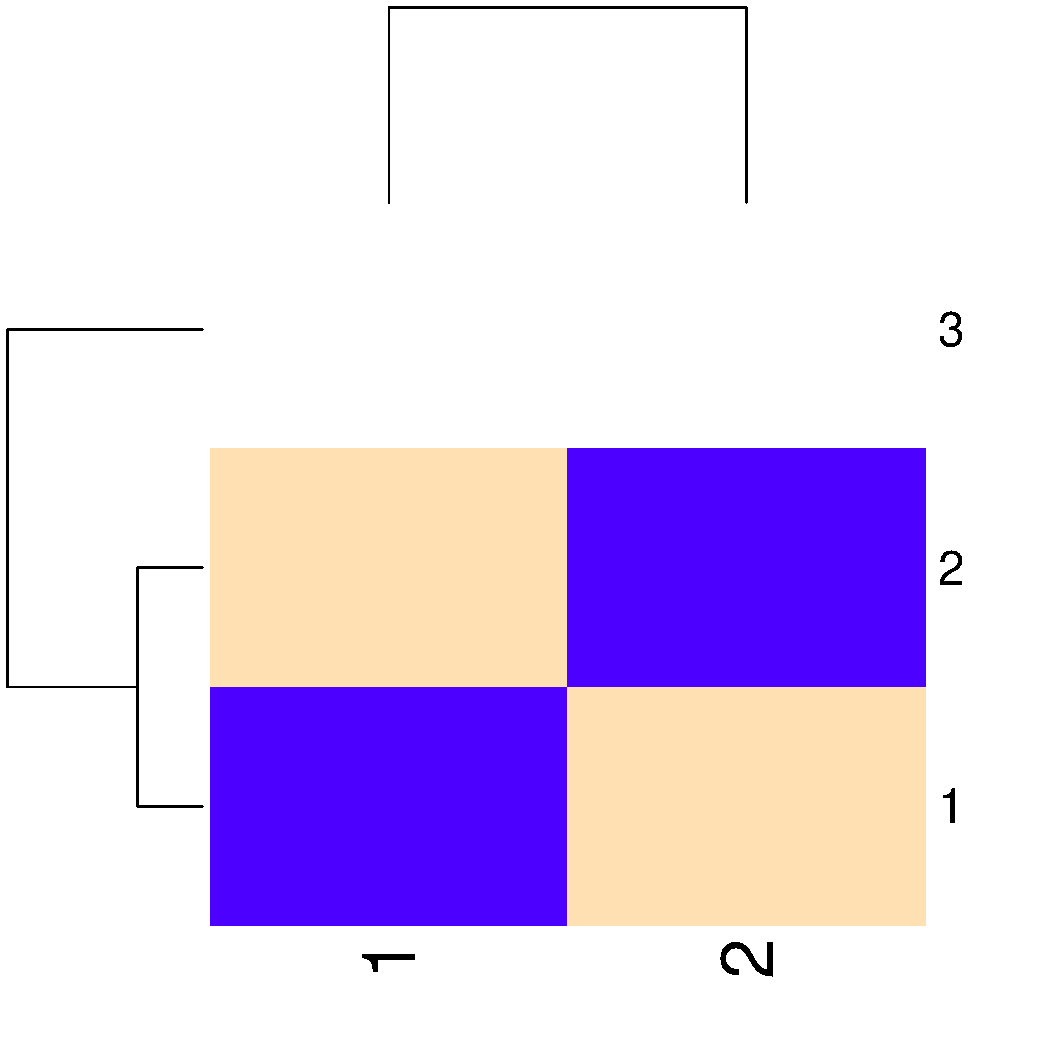
\includegraphics[width=\maxwidth]{figure/minimal-testing} 

}



\end{knitrout}


\begin{knitrout}
\definecolor{shadecolor}{rgb}{0.969, 0.969, 0.969}\color{fgcolor}\begin{kframe}
\begin{alltt}
\hlfunctioncall{jpeg}(\hlstring{"~/Desktop/03_Lotus_annotation/2013_week44/04_genelist.txt.arrayData.jpg"}, width = 2600, 
    height = 1800, quality = 90, units = \hlstring{"px"})
d <- \hlfunctioncall{read.table}(\hlstring{"~/Desktop/03_Lotus_annotation/2013_week44/04_genelist.txt.arrayData"}, header = T)
\hlcomment{# d_all <-}
\hlcomment{# read.table('~/Desktop/03_Lotus_annotation/2013_week44/export_2013-11-04-02-43-41_5411.txt.means',}
\hlcomment{# header=T) head(d) names(d) plot(d$Mean_WT_control1, d$Std_WT_control1)}
\hlcomment{# plot(d_all$Mean_WT_control1, d_all$Std_WT_control1, col='red')}
\hlcomment{# length(which(d_all$Std_WT_control1/d_all$Mean_WT_control1 >0.2))}
\hlfunctioncall{par}(mfcol = \hlfunctioncall{c}(1, 1), mar = \hlfunctioncall{c}(2.5, 2.5, 2.5, 2.5), oma = \hlfunctioncall{c}(25, 1, 1, 80))
d2 <- \hlfunctioncall{as.matrix}(d[, ])
\hlcomment{# seed - lightblue pod - blue flower - yellow shoot - green petiole - pink leaf - violet}
\hlcomment{# stem - white root - gray nodules - red nodules+root - orange}

colors <- \hlfunctioncall{c}(\hlfunctioncall{rep}(\hlstring{"lightblue"}, length = 5), \hlfunctioncall{rep}(\hlstring{"blue"}, length = 1), \hlfunctioncall{rep}(\hlstring{"yellow"}, length = 2), 
    \hlfunctioncall{rep}(\hlstring{"green"}, length = 30), \hlfunctioncall{rep}(\hlstring{"pink"}, length = 1), \hlfunctioncall{rep}(\hlstring{"violet"}, length = 2), \hlfunctioncall{rep}(\hlstring{"white"}, 
        length = 2), \hlfunctioncall{rep}(\hlstring{"gray"}, length = 28), \hlfunctioncall{rep}(\hlstring{"red"}, length = 5), \hlfunctioncall{rep}(\hlstring{"orange"}, length = 2))
\hlfunctioncall{heatmap}(d2, labRow = \hlfunctioncall{rownames}(d), labCol = \hlfunctioncall{c}(\hlfunctioncall{colnames}(d)), col = \hlfunctioncall{topo.colors}(100), keep.dendro = FALSE, 
    Colv = NA, cex.axis = 0.1, pch = 10, cex.lab = 1.1, cexRow = 2.5, cexCol = 1.5, ColSideColors = colors)
\hlfunctioncall{dev.off}()
\end{alltt}
\begin{verbatim}
## pdf 
##   2
\end{verbatim}
\end{kframe}
\end{knitrout}


\section{Plotting}


\end{document}
